\subsection{\texorpdfstring{SYSTEM OF TYPE \(E_{7}\)}{SYSTEM OF TYPE E\_7}}

\begin{enumerate}
\def\labelenumi{(\Roman{enumi})}
\tightlist
\item
  and (II) Let \(E = R^{8}\) , and let \(R_{8}\) be the root system in E constructed in no. 10. Let V be the hyperplane in E generated by the roots \(\alpha_{1}, \ldots, \alpha_{7}\) of \(R_{8}\) ; it is orthogonal to the eighth fundamental weight \(\omega = \varepsilon_{7} + \varepsilon_{8}\) of \(R_{8}\) .
\end{enumerate}

Let \(R = R_{8} \cap V\) . Then \(R\) is a reduced root system with basis \((\alpha_{1}, \ldots, \alpha_{7})\) , cf.~§ 1. no. 7, Cor. 4 of Prop. 20; hence, this system is of type \(E_{7}\) . Its elements are:

\[
\begin{array}{c} \pm \varepsilon_ {i} \pm \varepsilon_ {j} (1 \leqslant i < j \leqslant 6), \quad \pm (\varepsilon_ {7} - \varepsilon_ {8}), \\ \pm \frac {1}{2} (\varepsilon_ {7} - \varepsilon_ {8} + \sum_ {i = 1} ^ {8} (- 1) ^ {\nu (i)} \varepsilon_ {i}) \quad \text { with } \sum_ {i = 1} ^ {8} \nu (i) \text { odd }. \end{array}
\]

The number of roots is \(n = 2 + \binom{6}{2}.4 + 2^6 = 126\) . The positive roots are

\[
\pm \varepsilon_ {i} + \varepsilon_ {j} (1 \leqslant i <   j \leqslant 6). - \varepsilon_ {7} + \varepsilon_ {8},
\]

\[
\frac {1}{2} \left(- \varepsilon_ {7} + \varepsilon_ {8} + \sum_ {i = 1} ^ {6} (- 1) ^ {\nu (i)} \varepsilon_ {i}\right) \quad \text { with } \sum_ {i = 1} ^ {6} \nu (i) \text { odd }.
\]

\begin{enumerate}
\def\labelenumi{(\Roman{enumi})}
\setcounter{enumi}{2}
\item
  We have \(h = \frac{n}{l} = 18\) .
\item
  Let \(\tilde{\alpha} = \varepsilon_8 - \varepsilon_7 = 2\alpha_1 + 2\alpha_2 + 3\alpha_3 + 4\alpha_4 + 3\alpha_5 + 2\alpha_6 + \alpha_7\) , which is a root. The sum of its coordinates with respect to \((\alpha_i)\) is \(17 = h - 1\) . It is therefore the highest root. It is orthogonal to \(\alpha_i\) for \(2 \leqslant i \leqslant 7\) , and \((\tilde{\alpha}|\alpha_1) = 1\) . The completed Dynkin graph is
\end{enumerate}

\pandocbounded{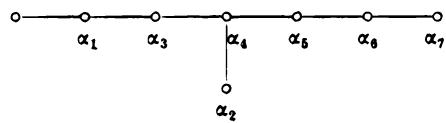
\includegraphics[keepaspectratio]{images/part002_8927380c.jpg}}

\begin{enumerate}
\def\labelenumi{(\Alph{enumi})}
\setcounter{enumi}{21}
\tightlist
\item
  Since \((\alpha |\alpha) = 2\) for all \(\alpha \in \mathbb{R}\) , we have \(R^{\prime} = R\) .
\end{enumerate}

For \(\Phi_{\mathrm{R}}\) , the squared length of the roots is \(\frac{1}{18}\) , so

\[
\Phi_ {\mathrm{R}} (x, y) = (x | y) / 36, \quad \text { and } \quad \gamma (\mathrm{R}) = 2 ^ {2}. 3 ^ {4}
\]

(§ 1. no. 12, formula (20)).

\begin{enumerate}
\def\labelenumi{(\Roman{enumi})}
\setcounter{enumi}{5}
\tightlist
\item
  Calculating the fundamental weights gives
\end{enumerate}

\[
\begin{array}{r l} & {\omega_ {1} = \varepsilon_ {8} - \varepsilon_ {7} = 2 \alpha_ {1} + 2 \alpha_ {2} + 3 \alpha_ {3} + 4 \alpha_ {4} + 3 \alpha_ {5} + 2 \alpha_ {6} + \alpha_ {7}} \\ & {\omega_ {2} = \frac {1}{2} (\varepsilon_ {1} + \varepsilon_ {2} + \varepsilon_ {3} + \varepsilon_ {4} + \varepsilon_ {5} + \varepsilon_ {6} - 2 \varepsilon_ {7} + 2 \varepsilon_ {8})} \\ & {\qquad = \frac {1}{2} (4 \alpha_ {1} + 7 \alpha_ {2} + 8 \alpha_ {3} + 12 \alpha_ {4} + 9 \alpha_ {5} + 8 \alpha_ {6} + 3 \alpha_ {7})} \\ & {\omega_ {3} = \frac {1}{2} (- \varepsilon_ {1} + \varepsilon_ {2} + \varepsilon_ {3} + \varepsilon_ {4} + \varepsilon_ {5} + \varepsilon_ {6} - 3 \varepsilon_ {7} + 3 \varepsilon_ {8})} \\ & {\qquad = 3 \alpha_ {1} + 4 \alpha_ {2} + 6 \alpha_ {3} + 8 \alpha_ {4} + 6 \alpha_ {5} + 4 \alpha_ {6} + 2 \alpha_ {7}} \\ & {\omega_ {4} = \varepsilon_ {3} + \varepsilon_ {4} + \varepsilon_ {5} + \varepsilon_ {6} + 2 (\varepsilon_ {8} - \varepsilon_ {7})} \\ & {\qquad = 4 \alpha_ {1} + 6 \alpha_ {2} + 8 \alpha_ {3} + 12 \alpha_ {4} + 9 \alpha_ {5} + 6 \alpha_ {6} + 3 \alpha_ {7}} \\ & {\omega_ {5} = \varepsilon_ {4} + \varepsilon_ {5} + \varepsilon_ {6} + \frac {3}{2} (\varepsilon_ {8} - \varepsilon_ {7})} \\ & {\qquad = \frac {1}{2} (6 \alpha_ {1} + 9 \alpha_ {2} + 12 \alpha_ {3} + 18 \alpha_ {4} + 15 \alpha_ {5} + 10 \alpha_ {6} + 5 \alpha_ {7})} \\ & {\omega_ {6} = \varepsilon_ {5} + \varepsilon_ {6} - \varepsilon_ {7} + \varepsilon_ {8}} \\ & {\qquad = 2 \alpha_ {1} + 3 \alpha_ {2} + 4 \alpha_ {3} + 6 \alpha_ {4} + 5 \alpha_ {5} + 4 \alpha_ {6} + 2 \alpha_ {7}} \\ & {\omega_ {7} = \varepsilon_ {6} + \frac {1}{2} (\varepsilon_ {8} - \varepsilon_ {7})} \\ & {\qquad = \frac {1}{2} (2 \alpha_ {1} + 3 \alpha_ {2} + 4 \alpha_ {3} + 6 \alpha_ {4} + 5 \alpha_ {5} + 4 \alpha_ {6} + 3 \alpha_ {7}).} \end{array}
\]

\begin{enumerate}
\def\labelenumi{(\Roman{enumi})}
\setcounter{enumi}{6}
\tightlist
\item
  The sum \(2\rho\) of the positive roots is \(2\sum_{i=1}^{7}\omega_i\) (§ 1. no. 10. Prop. 29), so
\end{enumerate}

\[
\begin{array}{r l} 2 \rho & = 2 \varepsilon_ {2} + 4 \varepsilon_ {3} + 6 \varepsilon_ {4} + 8 \varepsilon_ {5} + 10 \varepsilon_ {6} - 17 \varepsilon_ {7} + 17 \varepsilon_ {8} \\ & = 34 \alpha_ {1} + 49 \alpha_ {2} + 66 \alpha_ {3} + 96 \alpha_ {4} + 75 \alpha_ {5} + 52 \alpha_ {6} + 27 \alpha_ {7}. \end{array}
\]

\begin{enumerate}
\def\labelenumi{(\Roman{enumi})}
\setcounter{enumi}{7}
\tightlist
\item
  By no. 10 (VIII) and § 1, no. 10. Prop. 28, we have
\end{enumerate}

\[
\mathrm{Q} (\mathrm{R}) = \mathrm{Q} (\mathrm{R} _ {8}) \cap \mathrm{V} = \mathrm{L} _ {3} \cap \mathrm{V} \quad \text { and } \quad \mathrm{P} (\mathrm{R}) = p (\mathrm{P} (\mathrm{R} _ {8})) = p (\mathrm{L} _ {3}),
\]

where p denotes the orthogonal projection of E onto V. The group \(Q(R)\) has basis \((\alpha_{1},\ldots,\alpha_{7})\) : the group \(P(R)\) is generated by \(Q(R)\) and

\[
p (\alpha_ {8}) = \alpha_ {8} - \frac {1}{2} \omega .
\]

We have \(\omega\in\mathrm{P}(\mathrm{R}_{8})\) , \(\frac{1}{2}\omega\notin\mathrm{P}(\mathrm{R}_{8})\) , so \(2p(\alpha_{8})\in\mathrm{Q}(\mathrm{R})\) and \(p(\alpha_{8})\notin\mathrm{Q}(\mathrm{R})\) . Thus, \(\mathrm{P}(\mathrm{R})/\mathrm{Q}(\mathrm{R})\) is isomorphic to Z/2Z and is generated by, for example, the image of \(\omega_{7}\) .

The connection index is 2.

\begin{enumerate}
\def\labelenumi{(\Roman{enumi})}
\setcounter{enumi}{8}
\tightlist
\item
  The sequence of exponents of \(W(R)\) has 7 terms. The numbers 1, 5, 7, 11, 13, 17, coprime to \(h = 18\) , feature in this sequence. The last exponent \(m\) must be such that \(m + m = 18\) (Chap. V, § 6. no. 2, formula (2)). Hence, the sequence of exponents is
\end{enumerate}

\[
1, 5, 7, 9, 11, 13, 17.
\]

\begin{enumerate}
\def\labelenumi{(\Alph{enumi})}
\setcounter{enumi}{23}
\tightlist
\item
  From (IX) and Chap. V. § 6, no. 2, Cor. 1 of Prop. 3, it follows that the order of W(R) is
\end{enumerate}

\[
2. 6. 8. 10. 12. 14. 18 = 2 ^ {10}. 3 ^ {4}. 5. 7.
\]

\begin{enumerate}
\def\labelenumi{(\Roman{enumi})}
\setcounter{enumi}{10}
\item
  The only automorphism of the Dynkin graph is the identity, so \(\mathbf{A}(\mathbf{R}) = \mathbf{W}(\mathbf{R})\) and \(w_0 = -1\) .
\item
  \(\mathrm{P}(\mathrm{R}^{-})/\mathrm{Q}(\mathrm{R}^{-})\) has only one non-identity element. It interchanges the vertices corresponding to \(\alpha_{0}\) and \(\alpha_{7}\) , \(\alpha_{1}\) and \(\alpha_{6}\) , \(\alpha_{3}\) and \(\alpha_{5}\) , and leaves \(\alpha_{2}\) and \(\alpha_{4}\) fixed.
\end{enumerate}

